\section{Systematic Literature Review}
Il processo di conduzione dell'analisi della letteratura è stato condotto seguendo le linee guida definite da Kitchenham \cite{kitchenhamSLR}:
\begin{enumerate}
    \item Definizione del processo di ricerca
    \item Identificazione della ricerca
    \item Validazione della qualità degli studi selezionati
    \item Estrazione e sintesi dei dati
    \item Reporting della revisione
\end{enumerate}

\subsection{Processo di Ricerca}

Il processo di ricerca per la conduzione dell'analisi della letteratura include la pianificazione di cinque passaggi utili alla collezione della letteratura.

\subsubsection{Definizione dell'obiettivo di ricerca}
Al fine di poter estrarre una tassonomia che possa essere di riferimento per i professionisti del software AI, l'obiettivo di ricerca dell'analisi della letteratura include lo scopo di identificare la presenza, l'impatto e la severità di istanze che possono causare AI-Technical Debt.
Inoltre, prevede di collezionare informazioni riguardanti possibili strategie di identificazione e di mitigazione della minaccia tramite tecniche di refactoring.


\subsubsection{Definizione delle Research Questions}
Dall'obiettivo definito, quindi sono state formulate le seguenti research question(RQs):
\hfill \break
\begin{rqbox}
\textbf{RQ1.1:} Quali tipologie di Technical Debt sono presenti nei sistemi AI?
\end{rqbox}
Molte tipologie di technical debt presenti in letteratura non hanno una definizione chiara
e precisa che ne permetta l’identificazione diretta nella pratica. È necessario, quindi,
seguire una strada analoga al lavoro introdotto da Ward Cunningham per la definizione
del Technical Debt \cite{Cunningham1992td}.
\hfill \break
\begin{rqbox}
\textbf{RQ1.2:} Quali sono gli approcci o i tool per identificare e mitigare TD nei sistemi AI?
\end{rqbox}
Al fine di fornire un metodo di riconoscimento ai professionisti del software AI delle istanze che possono causare technical debt, è necessario ricerca approcci che possano favorire l'identificazione. Questa parte del lavoro ha maggior successo se questi approcci sono stati implementati e distribuiti tramite la realizzazione di possibili tool, permettendo agli utenti della tassonomia di avere una tecnica automatizzata per l'identificazione.
Allo stesso modo, al fine di poter creare una linea guida utile ai professionisti del software AI, il lavoro di tesi si pone di ricercare possibili tecniche di refactoring utili a mitigare o ridurre il technical debt nei sistemi AI.

\subsubsection{Definizione del Coding Schema}

Al fine di pianificare lo schema di informazioni utile a indirizzare l'estrazione dei dati è necessario definire un processo di coding.
Il coding è il processo che comprende l'organizzazione di un grande ammontare di dati in piccoli frammenti, che favorisce l'estrazione delle informazioni.
Il processo prevede quindi l'assegnazione di codici, parole chiavi o frasi che identificano a quale problema o a quale argomento si riferiscono \cite{bailey2017guide}. 

La pianificazione del coding per il presente lavoro di tesi prevede innanzitutto la definizione di un coding schema preliminare, ossia un insieme di codici estratti dall'obiettivo di ricerca e dalle research questions formulate al fine di indirizzare la ricerca. Lo schema risultante deve poi essere verificato e raffinato attraverso l'applicazione dello schema su un sottoinsieme di articoli, così da ritrovare eventuali codici ancora non inclusi.
Il coding schema pianificato è definito in Tabella \ref{tab:coding_schema}.

\begin{table}[h!]
    \centering
    \begin{tabular}{|c|p{6cm}|}
        \multicolumn{2}{c}{\textbf{Coding schema}} \\
        
        \hline
        Scopo o topic & Informazioni relative allo scopo su cui opera l'articolo e il suo contributo di ricerca. \\
        \hline
        Tipologia di risorsa & Conferenza, Workshop o Journal e la tipologia dell'articolo.\\
        \hline
        Lista di istanze di technical Debt & Elenco dei nomi utilizzati per rappresentare le istanze di technical debt.\\
        \hline
        Definizioni di technical debt & Per ogni istanza riscontrata, definizione di essa. \\
        \hline
        Strategia di identificazione & Informazioni sulle strategie di identificazione delle istanze di technical debt. \\
         \hline
        Strategia di refactoring & Informazioni sulle strategie di refactoring delle istanze di technical debt. \\
         \hline
        Strumenti di identificazione & Informazioni sugli strumenti di identificazione delle istanze di technical debt. \\
        \hline
        Strumenti di refactoring & Informazioni sugli strumenti di refactoring delle istanze di technical debt. \\
        \hline
        Note & Informazioni aggiuntive non raggiungibili dal coding schema. \\
        \hline
    \end{tabular}
    \caption{Coding Schema pianificato per la Systematic Literature Review}
    \label{tab:coding_schema}
\end{table}


\subsubsection{Definizione del protocollo di revisione}
La revisione della letteratura prevede quindi una serie di attività che, a partire dalle sorgenti di dati, sarà possibile estrarre la serie di articoli che sono strettamente relativi all'obiettivo di ricerca definito.
Il protocollo di revisione quindi è utile alla conduzione sistematica della revisione per fornire una metodologia di selezione degli studi primari. La Figura \ref{fig:slr_process} definisce il protocollo di revisione adoperato per condurre lo studio, basato sulle linee guida definite da Kitchenham \cite{kitchenhamSLR}.
\begin{figure}
    \centering
    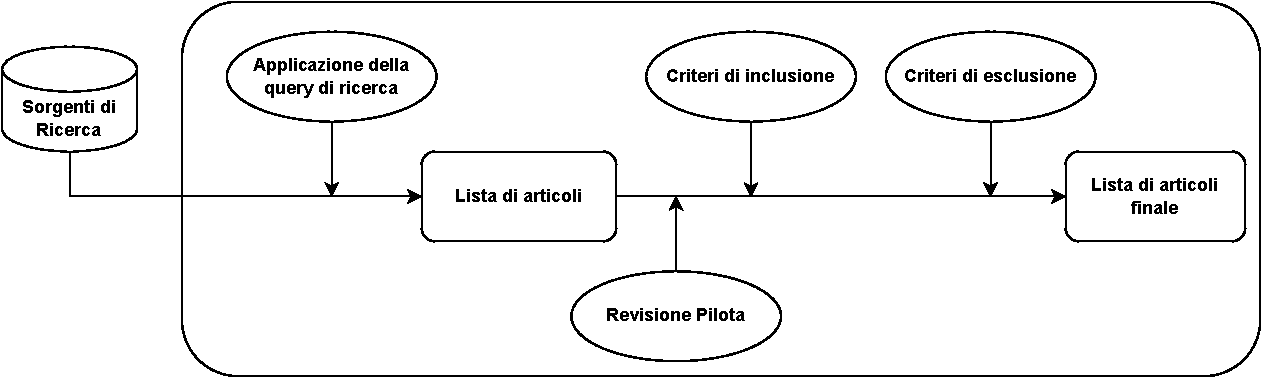
\includegraphics[width=1\textwidth]{Figure/Design/review_process.pdf}
    \caption{Protocollo di revisione della letteratura}
    \label{fig:slr_process}
\end{figure}
\subsection{Identificazione della Ricerca}
In questa sezione sono definiti le tecniche e le strategie utili alla selezione e la revisione degli articoli, seguendo il protocollo di revisione.
\subsubsection{Strategia di ricerca}
%sorgenti e search query
La strategia di ricerca include lo schema che definisce l'insieme delle sorgenti da analizzare, i termini di ricerca rilevanti, la definizione dei criteri di inclusione e di esclusione e infine la query di ricerca utilizzata.

Per questo lavoro sono state selezionate la lista di sorgenti bibliografiche rilevanti come suggerito da Kitchenham and Charters, definite anche come le più rappresentative del dominio di ingegneria del software \cite{Kitchenham2007}.
La lista include quindi: ACM Digital Library, IEEEXplore Digital Library, Web of Science e Scopus.

I termini di ricerca sono stati collezionati per poter rappresentare due sottogruppi di terminologie: una rappresentante le diverse tipologie di technical debt, l'altra rappresentante le diverse terminologie utilizzate per indicare l'intelligenza artificiale. La combinazione di questi due sottogruppi ha portato poi alla formulazione della seguente \textit{search query}:
\begin{quote}
   ("technical debt" $\vee$ "tech debt" $\vee$ "requirements debt" $\vee$ "data debt" $\vee$ "data smell*" $\vee$ "code debt" $\vee$ "build debt" $\vee$ "model debt" $\vee$ "documentation debt" $\vee$ "versioning debt" $\vee$ "defect debt" $\vee$ "configuration debt" $\vee$ "infrastructure debt" $\vee$ "design debt" $\vee$ "architecture debt" $\vee$ "architectural debt" $\vee$ "test debt" $\vee$ "defect debt" $\vee$ "abstraction debt" $\vee$ "ethics debt" $\vee$ "analysis debt" $\vee$ "" $\vee$ antipattern* $\vee$ anti-pattern* $\vee$ smell*) $\wedge$ ("machine learning" $\vee$ "deep learning" $\vee$ ai $\vee$ ml $\vee$ dl $\vee$ "artificial intelligence")
\end{quote}
E' stato utilizzato il carattere $"*"$ per indicare la possibile variazione dei termini (\eg variazione del termine da singolare a plurale).
Per incrementare la rilevanza degli articoli riscontrati, la search query è stata utilizzata sia sull'analisi del titolo sia sull'analisi dell'abstract dell'articolo.

\subsubsection{Definizione degli criteri di inclusione e esclusione}
Sono stati definiti i criteri di inclusione da essere applicati sia durante la fase di revisione iniziale in cui viene analizzato titolo e abstract dell'articolo (T\&A) sia durante la fase di revisione completa (F), come illustrato in Tabella \ref{tab:criteria}.

\begin{table}[h!]
    \centering
    \begin{tabular}{|c|p{6cm}|p{1.6cm}|}
    \hline
    \textbf{Criteria} & \textbf{Criterio di valutazione} & \textbf{Fase} \\ \hline 
    \multirow{2}{*}{\textbf{Inclusion}} & (I1) Articoli che definiscono le tipologie di technical Debt nei sistemi AI & Entrambi \\ \cline{2-3} 
    & (I2) Articoli che presentano approcci alla identificazione di technical Debt nei sistemi AI & Entrambi  \\\cline{2-3} 
    & (I3) Articoli che presentano approcci alla mitigazione di technical debt nei sistemi AI & Entrambi \\ \cline{2-3} 
    & (I4) Articoli che presentano tool per la identificazione di technical debt nei sistemi AI & Entrambi \\\cline{2-3}  
    & (I5) Articoli che presentano tool per la mitigazione di technical debt nei sistemi AI & Entrambi \\ \hline 
    \multirow{2}{*}{\textbf{Exclusion}} & (E1) Articoli non scritti interamente in lingua inglese & T\&A\\ \cline{2-3} 
    & (E2) Articoli che non stati soggetti a una peer review (i.e., blog, forum, book, book chapter, ...) &  T\&A\\ \cline{2-3} 
    & (E3) Articoli duplicati (da considerare solo la versione più recente) & T\&A \\ \cline{2-3} 
    & (E4) Position papers e work plans (i.e., articoli che non riportano risultati) & T\&A \\ \cline{2-3} 
    & (E5) Pubblicazioni non accessibili & T\&A \\ \hline
    \end{tabular}
    \caption{Criteri di inclusione e esclusione degli articoli in letteratura }
    \label{tab:criteria}
\end{table}

\subsection{Validazione della qualità degli studi selezionati}
Al fine di migliorare la qualità della metodologia di revisione adoperata, sono state utilizzate delle tecniche di validazione.
Per ridurre il fattore di soggettività all'interno del processo, è stato incluso un processo di \textit{Inter-rater assessment}.
In dettaglio, per la revisione è stata condotta da tre ricercatori, esperti di Technical Debt per i sistemi AI, al fine di valutare la search query e i criteri di inclusione e esclusione.
Il processo di revisione ha previsto un'analisi iniziale condotta da ogni ricercatore analizzando, tramite l'utilizzo dei criteri di inclusione ed esclusione, il titolo e l'abstract di ogni articolo.
A ogni articolo, quindi, viene assegnata la revisione da parte di due ricercatori, i quali dovranno esprimere il loro giudizio per l'inclusione (assegnato tramite il valore 1) o l'esclusione (assegnato tramite il valore 0).
In caso di disaccordo tra le valutazioni, è stato coinvolto il terzo ricercatore al fine di esprimere il voto finale.
Successivamente, è stato condotto un test pilota su un sottoinsieme di 6 articoli, revisionato da coppie di ricercatori.
Questo ultimo step ha permesso quindi di poter valutare la bontà del processo definito e di poter ottimizzare e raffinare i dettagli.

